\documentclass[a4paper, 11pt]{article}
\usepackage{comment}
\usepackage{lipsum} 
\usepackage{fullpage} %cambiar margen
\usepackage[a4paper, total={7in, 10in}]{geometry}

\usepackage{amssymb,amsthm} 
\usepackage{amsmath}
\newtheorem{theorem}{Theorem}
\newtheorem{corollary}{Corollary}
\usepackage{graphicx}
\usepackage{tikz}
\usetikzlibrary{arrows}
\usepackage{verbatim}
%\usepackage[numbered]{mcode}
\usepackage{float}
\usepackage{tikz}
\usetikzlibrary{shapes,arrows}
\usetikzlibrary{arrows,calc,positioning}
\usepackage{mathpazo} %tipo de letra 
\usepackage[utf8]{inputenc} %codificación
\usepackage[T1]{fontenc} %digitación de tildes y ñ
\usepackage[spanish]{babel} %paquete de soporte español

\tikzset{
	block/.style = {draw, rectangle,
		minimum height=1cm,
		minimum width=1.5cm},
	input/.style = {coordinate,node distance=1cm},
	output/.style = {coordinate,node distance=4cm},
	arrow/.style={draw, -latex,node distance=2cm},
	pinstyle/.style = {pin edge={latex-, black,node distance=2cm}},
	sum/.style = {draw, circle, node distance=1cm},
}
\usepackage{xcolor}
\usepackage{mdframed}
\usepackage[shortlabels]{enumitem}
\usepackage{indentfirst}
\usepackage{hyperref}

\usepackage{listings}
\lstset{literate=
  {á}{{\'a}}1
  {é}{{\'e}}1
  {í}{{\'i}}1
  {ó}{{\'o}}1
  {ú}{{\'u}}1
  {Á}{{\'A}}1
  {É}{{\'E}}1
  {Í}{{\'I}}1
  {Ó}{{\'O}}1
  {Ú}{{\'U}}1
  {ñ}{{\~n}}1
  {ü}{{\"u}}1
  {Ü}{{\"U}}1
}

\lstdefinestyle{customc}{
  belowcaptionskip=1\baselineskip,
  breaklines=true,
  frame=L,
  xleftmargin=\parindent,
  language=Python,
  showstringspaces=false,
  basicstyle=\footnotesize\ttfamily,
  keywordstyle=\bfseries\color{green!40!black},
  commentstyle=\itshape\color{purple!40!black},
  identifierstyle=\color{blue},
  stringstyle=\color{orange},
}

\lstdefinestyle{customasm}{
  belowcaptionskip=1\baselineskip,
  frame=L,
  xleftmargin=\parindent,
  language=[x86masm]Assembler,
  basicstyle=\footnotesize\ttfamily,
  commentstyle=\itshape\color{purple!40!black},
}

\lstset{escapechar=@,style=customc}



\renewcommand{\thesubsection}{\thesection.\alph{subsection}}

\newenvironment{problem}[2][Ejercicio]
{ \begin{mdframed}[backgroundcolor= red!50] \textbf{#1 #2} \\}
	{  \end{mdframed}}

% Define solution environment
\newenvironment{solution}
{\textcolor{blue}{\textbf{\textit{Solución:\\\noindent}}}}


\renewcommand{\qed}{\quad\qedsymbol}

% \\	
\begin{document}
	\noindent
	%%%%%%%%%%%%%%%%%%%%%%%%%%%%%%%%%%%%
	
	\begin{minipage}[b][1.2cm][t]{0.8\textwidth}
		\large\textbf{César Isaí García Cornejo} \hfill \textbf{Tarea 8}  \\
		cesar.cornejo@cimat.mx \hfill \\
		\normalsize Computo Científico \hfill Semestre 3\\
	\end{minipage}
	
	\hspace{14.4cm}
	\begin{minipage}[b][0.03cm][t]{0.12\linewidth}
		
		\vspace{-2.2cm}
		%%%La Ruta dependerá de donde este alojado el main y la imagen
		
\includegraphics[scale=0.3]{Figures/EscudoCimat.png}
	\end{minipage}
	
	\noindent\rule{7in}{2.8pt}
	
	%%%%%%%%%%%%%%%%%%%%%
	%%%%%%%%%%%%%%%%%%%%%%%%%%%%%%%%%%%%%%%%%%%%%%%%%%%%%%%%%%%%%%%%%%%%%%%%%%%%%%%%%%%%%%%%%%%%%%%%%%%%%%%%%%%%%%%%%%%
	% Problem 1
	%%%%%%%%%%%%%%%%%%%%%%%%%%%%%%%%%%%%%%%%%%%%%%%%%%%%%%%%%%%%%%%%%%%%%%%%%%%%%%%%%%%%%%%%%%%%%%%%%%%%%%%%%%%%%%%%%%%%%%%%%%%%%%%%%%%%%%%%
	\setlength{\parskip}{\medskipamount}
	\setlength{\parindent}{0pt}
%/////////// Ejercicio 1 /////////////////

\begin{problem}{1} 
    Aplique el algoritmo de Metropolis-Hastings considerando como función objetivo la distribución normal bivariada:
    \begin{align*}
      f_{X_1,X_2}(\bar{x}) = \frac{1}{2\pi} |\Sigma|^{-1/2} \exp \left \{ -\frac{1}{2} (\bar{x} - \mu)' \Sigma^{-1}(\bar{x} - \mu) \right \}
    \end{align*}
    donde,
    \begin{align*}
      \mu = \binom{\mu_1}{\mu_2}, \:\:\:\: \Sigma = 
      \begin{pmatrix}
        \sigma_1^2 &  \rho \sigma_1 \sigma_2\\
        \rho \sigma_1 \sigma_2 & \sigma_2^2
      \end{pmatrix}
    \end{align*}
    Así se tienen las siguientes distribuciones condicionales: 
    \begin{align*}
      X_1|X_2 &= x_2 \sim N \left(\mu_1 + \rho \frac{\sigma_1 }{\sigma_2}(x_2 - \mu_2 )\:,\: \sigma_1^2 (1-\rho^2)\right)\\
      X_2|X_1 &= x_1 \sim N \left(\mu_1 + \rho \frac{\sigma_2 }{\sigma_1}(x_1 - \mu_1 )\:,\: \sigma_2^2 (1-\rho^2)\right)
    \end{align*}
    Considere las siguientes propuestas: 
    \begin{align*}
      q_1((x_1',x_2')|(x_1,x_2)) = f_{X_1|X_2}(x'_1|x_2)I(x'_2= x_2)\\
      q_2((x_1',x_2')|(x_1,x_2)) = f_{X_2|X_1}(x'_2|x_1)I(x'_1= x_1)
    \end{align*}
    A partir del algoritmo MH usando Kerneles híbridos simule valores de la distribución normal bivariada, fijando $\sigma_1 = \sigma_2=1$, considere los casos $\rho = $ 0.8 y $\rho = $ 0.95. 

\end{problem}
  
\begin{solution} 
  
  Observemos que tenemos como distribuciones propuestas justamente las distribuciones condicionales de la distribución objetivo que es la normal bivariada. Ya hemos probado, el el caso general que estas son propuestas de Gibbs. Por tanto, tenemos que la cadena de Markov acepta con probabilidad uno cada propuesta. Luego, el método de Metropolis-Hastings se reduce a tomar realizaciones de las densidades condicionales según un kernel híbrido. Dicho kernel se diseño para que con probabilidad de un medio simule de la primer coordenada (eje x) mientras que con el resto de probabilidad simula de la condicional para la segunda coordenada (eje y). 

  Además, con el fin de tener una cadena fuertemente aperiodica, en la implementación se creo un paso extra que ocurre con probabilidad de $10^{-5}$ de quedarse en el mismo punto de la cadena.

  Los resultados de dichas implementaciones se muestran a continuación. Para el caso con correlación $\rho =$ 0.80
  \begin{figure}[H] 
      \centering 
      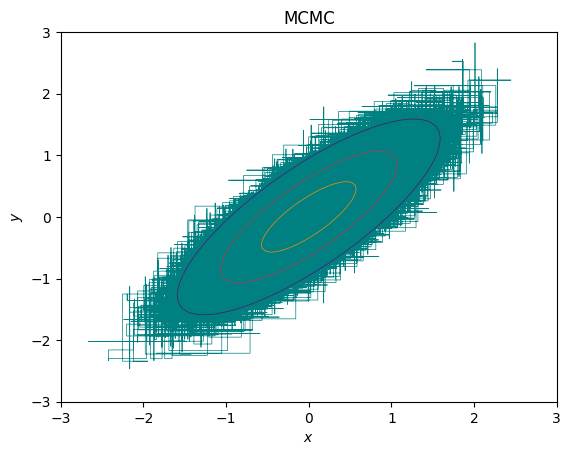
\includegraphics[width = 10 cm]{Figures/hibrido1.png} 
      \caption{Trayectoria de la simulación de la normal bivariada con correlación 0.8}
      \label{Fig. 1.01}
  \end{figure} 

  Para la simulación de la normal bivariada con $\rho =$ 0.95
  \begin{figure}[H] 
      \centering 
      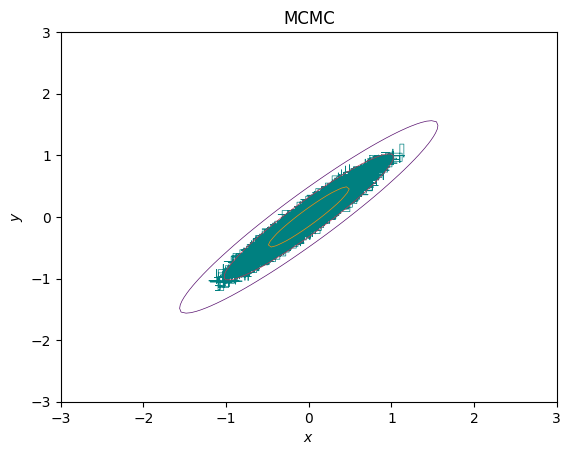
\includegraphics[width = 10 cm]{Figures/hibrido2.png} 
      \caption{Trayectoria de la simulación de la normal bivariada con correlación 0.95}
      \label{Fig. 1.02}
  \end{figure} 

  Nótese que tenemos el comportamiento esperado en cada caso, primero vemos que al aumentar la correlación tenemos un adelgazamiento de la elipse. Luego, la trayectoria cubre satisfactoriamente las curvas de nivel de la gráfica de la normal bivariada.

  Observemos por completitud que efectivamente las marginales distribuyen normales, como vemos en los siguientes gráficas
  \begin{figure}[H] 
      \centering 
      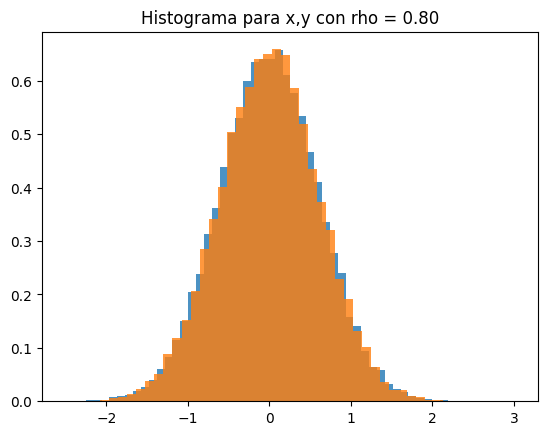
\includegraphics[width = 10 cm]{Figures/histograma_1_1.png} 
      \caption{Histograma de cada componente para $\rho = 0.80$}
      \label{Fig. 1.03}
  \end{figure} 
  \begin{figure}[H] 
      \centering 
      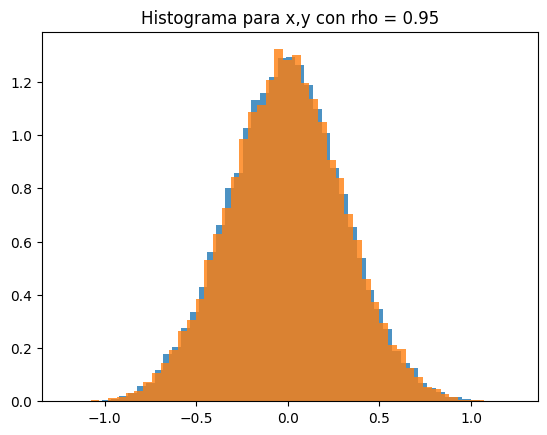
\includegraphics[width = 10 cm]{Figures/histograma_1_2.png} 
      \caption{Histograma de cada componente para $\rho = 0.95$}
      \label{Fig. 1.04}
  \end{figure} 
  lo que concluye el análisis.

\end{solution}
  



\begin{problem}{2} 
  Considere los tiempos de falla $t_1,...,t_n$ con distribución $Weibull(\alpha,\lambda)$:
    \begin{align*}
      f(t_i|\alpha,\lambda) = \alpha \lambda t_i^{\alpha-1} e^{-t_i^{\alpha}\lambda}
    \end{align*}
    Se asumen como a priori $\alpha \sim exp(c)$ y $\lambda|\alpha \sim Gama(\alpha,b)$, por tanto, $f(\alpha, \lambda) = f(\lambda|\alpha)f(\alpha)$. Así, para la distribución posterior se tiene:
    \begin{align*}
      f(\alpha,\lambda|\bar{t}) \propto f(\bar{t}|\alpha, \lambda)f(\alpha,\lambda) 
    \end{align*}
    A partir del algoritmo MH usando Kerneles híbridos simule valores de la distribución posterior $f(\alpha, \lambda|\bar{t})$, considerando la siguientes propuestas:
    \begin{enumerate}[a)]
      \item Propuesta: 
      \begin{align*}
        \lambda_p |\alpha, \bar{t} \sim Gama \left(\alpha + n , b + \sum_{i = 1 }^{n}t_i^{\alpha}\right) \:\:\:\: \text{y dejando $\alpha$ fijo.} 
      \end{align*}
      \item Propuesta:
      \begin{align*}
        \alpha_p|\lambda, \bar{t} \sim Gama(n+1, -\log(b)-\log(r_1)+c), \text{ con }  r_1 = \prod_{i=1}^{n}t_i \text{ y dejando $\lambda$ fijo.}
      \end{align*}
      \item Propuesta:
      \begin{align*}
        \alpha_p \sim exp(c) \text{ y } \lambda_p |\alpha_p \sim Gama(\alpha_p,b).
      \end{align*}
      \item Propuesta:
      \begin{align*}
        \alpha_p = \alpha + \varepsilon \sim N(0,\sigma) \text{ y dejando $\lambda$ fijo.} 
      \end{align*}
      Simular datos usando $\alpha = 1$ y $\lambda =1$ con $n = 20$. Para la priori usar $c= 1$ y $ b = 1$.
    \end{enumerate}

\end{problem}
  
\begin{solution} 
  
La distribución objetivo es la distribución posterior que se obtiene directamente con el cálculo:
\begin{align*}
  f(\alpha, \lambda| \bar{t}) \propto  \prod_{i = 1}^{n} \left(\alpha \lambda t-i^{\alpha -1} e^{t_i^\alpha \lambda}\right) \cdot \frac{b^\alpha}{\Gamma(\alpha)} \lambda^{\alpha -1} e^{-\lambda b} \cdot c e^{-\alpha c} 
\end{align*}
para $\alpha >0$ y $\lambda > 0$. Simplificando
\begin{align*}
  f(\alpha, \lambda, \bar{t} ) \propto \lambda^{n+\alpha -1} e^{-\lambda(b + \sum t_i^\alpha) } \cdot \frac{\left(b\prod_{i=1}^{n} t_I\right)^\alpha }{\Gamma(\alpha)} \alpha^{n} e^{-\alpha c}
\end{align*}
De aquí es claro que la marginal de $\lambda$ sigue una distribución gama, es decir
\begin{align*}
  \lambda_p|\alpha \sim Ga(n+ \alpha, b + \sum_{i = 1}^{n} t_i^\alpha) 
\end{align*}
que coincide con la primer propuesta dada por en enunciado del ejercicio. Por tanto, dicha propuesta es propuesta de Gibbs.

Nuevamente, implementamos el método de Metropolis-Hastings para kernel híbrido. El primer kernel, como vimos, es un kernel de Gibbs. Luego, cada propuesta se acepta siempre. Sin embargo, el segundo kernel tiene un problema, pues al tomar $ b= 1, c=1$, tenemos que es necesario que $\sum_{i = 1}^{n} \log t_i < 1$ para tener parámetro positivo. Luego, dicha condición no es frecuente, por lo que se decidió por descartar o rechazar cada propuesta donde no se satisfaga. La siguiente propuesta tiene \textit{actualizaciones} en ambos parámetros y se basa en una Metropolis-Hastings convencional, con propuesta no simétrica. El último kernel es una camina aleatoria solo en el parámetro $\alpha$ 

La grafica de la trayectoria dada por la simulación es 
\begin{figure}[H] 
    \centering 
    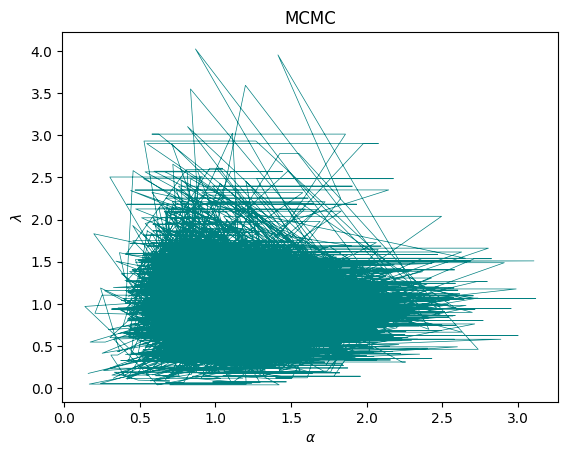
\includegraphics[width = 10 cm]{Figures/trayectoria_2.png} 
    \caption{Trayectoria de la cadena por MCMC.}
    \label{Fig. 2.01}
\end{figure} 

Los kerneles en este caso se decidió tomar no equiprobable ya que las simulaciones del segundo kernel aumentan considerablemente los valores de $\lambda$. 

Para ver los resultados más claramente, obtenemos los histogramas de cada componente
\begin{figure}[H] 
    \centering 
    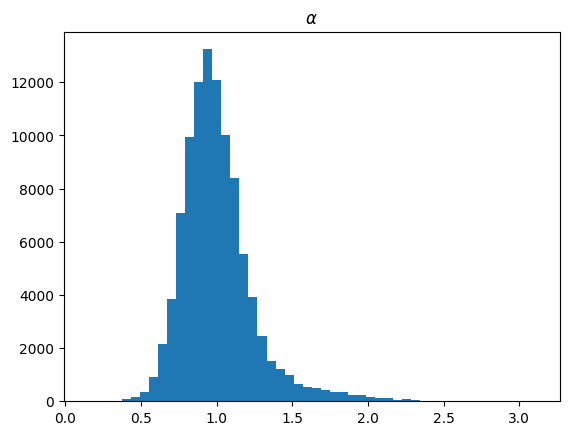
\includegraphics[width = 10 cm]{Figures/histograma_2_alpha.png} 
    \caption{Histograma para la marginal $\alpha$ de la posterior.}
    \label{Fig. 2.02}
\end{figure} 
\begin{figure}[H] 
    \centering 
    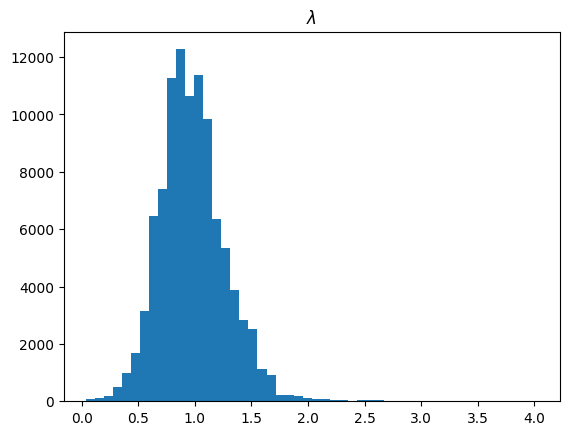
\includegraphics[width = 10 cm]{Figures/histograma_2_lambda.png} 
    \caption{Histograma para la marginal $\lambda$ de la posterior.}
    \label{Fig. 2.03}
\end{figure} 

Para obtener una estimación puntual de los valores de $\alpha$ y $\lambda$ simplemente tomamos la media, que nos dá
\begin{lstlisting}
Media muestral para alpha:  1.0079571771956224
Media muestral para lambda: 0.9836892081931157
\end{lstlisting}
Luego, tenemos una estimación posterior considerable para la distribución de los datos, pues recordemos que dichos datos son realizaciones de la Weibull($\alpha = 1, \lambda= 1$).




\end{solution}



\begin{problem}{3} 
  Considera el ejemplo referente al número de fallas en bombas de agua en una central nuclear, donde $p_i$ representa el número de fallas en el tiempo de operación $t_i$, con $i = 1,...,n$.

  Considera el modelo $p_i \sim Poisson(\lambda_i t_i)$, (las $\lambda_i$ son independientes entre si), con distribuciones a priori $\lambda_i |\beta \sim Gama(\alpha,\beta)$ y $ \beta \sim Gama(\gamma,\delta)$, por tanto:
  \begin{align*}
    f(\lambda_1,...,\lambda_n,\beta) = f(\lambda_1,\beta)f(\lambda_2,\beta)\cdots f(\lambda_n,\beta)f(\beta)
  \end{align*}
  Para la distribución posterior se tiene: 
  \begin{align*}
    f(\lambda_1,...,\lambda_n,\beta|\bar{p}) \propto L(\bar{p}, \bar{\lambda},\beta)f(\lambda_1,...,\lambda_n,\beta)
  \end{align*}
  Simule valores de la distribución posterior $f(\lambda_1,...,\lambda_n,\beta|\bar{p})$, usando un kernel híbrido, considerando las propuestas:
  \begin{align*}
    \lambda_i|\bar{\lambda_{-i}},\beta,\bar{t} \sim Gama(p_i + \alpha, \beta +t_i)\\
    \beta| \bar{\lambda}, \bar{t} \sim Gama \left(n\alpha + \gamma , \delta + \sum_{i=1}^{n}\lambda_i\right) .
  \end{align*}
  Verifique que estas son propuestas Gibbs.
  Use los datos del cuadro 1 con los parámetros a priori $\alpha = $ 1.8, $\gamma = $ 0.01 y $\delta = 1$.
\end{problem}


\begin{solution} 
  Empezaremos por mostrar que en efecto la propuesta correspondiente son propuestas de Gibbs. Consideremos la verosimilitud
  \begin{align*}
    \mathcal{L}(\bar{p},\lambda,\beta) = \prod_{i = 1}^{n} \frac{(\lambda_i p_i)^{p_i}}{p_i!}e^{-\lambda_i t_i}
  \end{align*}
  Por tanto, la distribución posterior es
  \begin{align*}
    f(\lambda_1, \cdots, \lambda_n,\beta|\bar{p}) &\propto \mathcal{L}(\bar{p},\bar{\lambda},\beta) f(\lambda_1,\cdots,\lambda_n,\beta)\\
    & \propto \mathcal{L}(\bar{p},\bar{\lambda},\beta) f(\lambda_1,\beta)f(\lambda_2,\beta)\cdots f(\lambda_n,\beta)f(\beta)\\
    &\propto \left(\prod_{i} \lambda_i^{p_i}\right) e^{-\sum_{i} \lambda_i t_i} \cdot \frac{\beta^\alpha}{\Gamma(\alpha)} \lambda_1 ^{\alpha-1} e^{-\beta \lambda_1} \cdots \frac{\beta^\alpha}{\Gamma(\alpha)} \lambda_n ^{\alpha-1} e^{-\beta \lambda_n}\cdot \beta^{\gamma-1} e^{-\delta \beta}
  \end{align*}
  Agrupando a cada término tenemos que 
  \begin{align*}
    f(\lambda_1, \cdots, \lambda_n,\beta|\bar{p}) & \propto \left(\prod_{i} \lambda_i^{p_i}\right) e^{-\sum_{i} \lambda_i t_i} \cdot \lambda_1 ^{\alpha-1} e^{-\beta \lambda_1} \cdots  \lambda_n ^{\alpha-1} e^{-\beta \lambda_n}\cdot \beta^{n\alpha +\gamma-1} e^{-\delta \beta}\\
    & \propto \left(\prod_{i} \lambda_i^{p_i}\right) e^{-\sum_{i} \lambda_i t_i} \cdot \lambda_1 ^{\alpha-1} \cdots  \lambda_n ^{\alpha-1} \cdot \beta^{n\alpha +\gamma-1} e^{-(\delta + \sum \lambda_i )\beta}\\
    & \propto \lambda_1 ^{p_1 + \alpha-1} e^{-(t_1 + \beta)\lambda_1}\cdots \lambda_n ^{p_n + \alpha-1} e^{-(t_n + \beta)\lambda_n}\cdot \beta^{n\alpha + \gamma-1} e^{-(\delta + \sum \lambda_i )\beta}
  \end{align*}

  De aquí, tomando las marginales es claro que $\lambda_i|\lambda_{-i},\beta, \bar{t} \sim Gama(p_i + \alpha, \beta + t_i)$ y con el último término tenemos que $\beta|\bar{\lambda},\bar{t} \sim Gama(n \alpha + \gamma, \delta + \sum \lambda_i)$. 

  Ahora, nos enfocaremos en los resultados de la implementación. Tras usar el método de Metropolis-Hastings con el kernel híbrido, donde cada kernel es equiprobable, tenemos que tras 100000 iteraciones los siguientes histogramas de las distribuciones marginales para cada componte de la distribución objetivo. Nótese que tenemos una distribución objetivo en 11 dimensiones
  \begin{figure}[H] 
      \centering 
      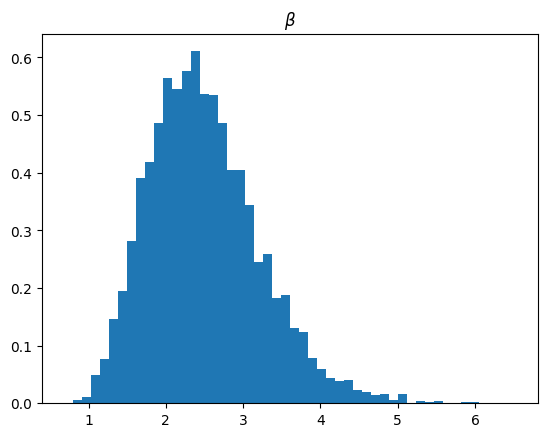
\includegraphics[width = 10 cm]{Figures/histograma3_beta.png} 
      \caption{Histograma de la marginal de la posterior de $\beta$.}
      \label{Fig. 3.01}
  \end{figure} 
  \begin{figure}[H] 
    \centering 
    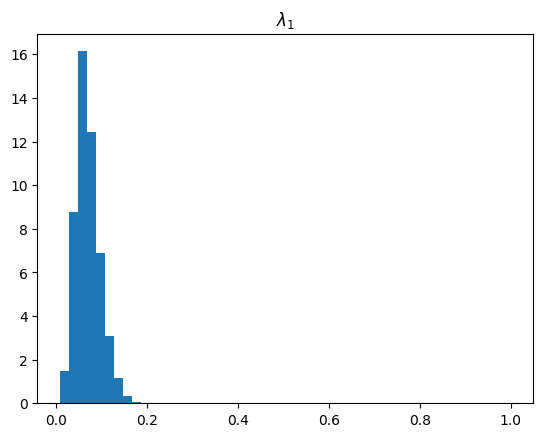
\includegraphics[width = 10 cm]{Figures/histograma3_1.png} 
    \caption{Histograma de la marginal de la posterior de $\lambda_1$.}
    \label{Fig. 3.02}
\end{figure} 
\begin{figure}[H] 
  \centering 
  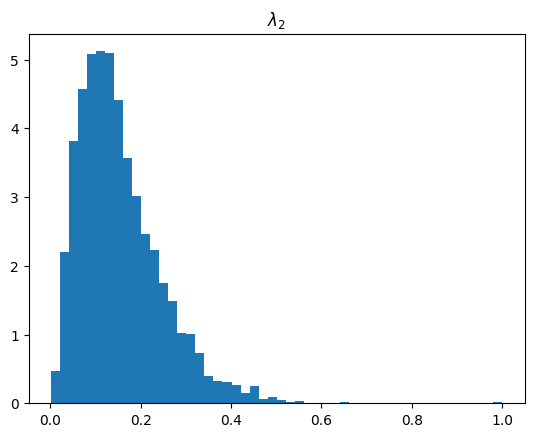
\includegraphics[width = 10 cm]{Figures/histograma3_2.png} 
  \caption{Histograma de la marginal de la posterior de $\lambda_2$.}
  \label{Fig. 3.03}
\end{figure} 
\begin{figure}[H] 
  \centering 
  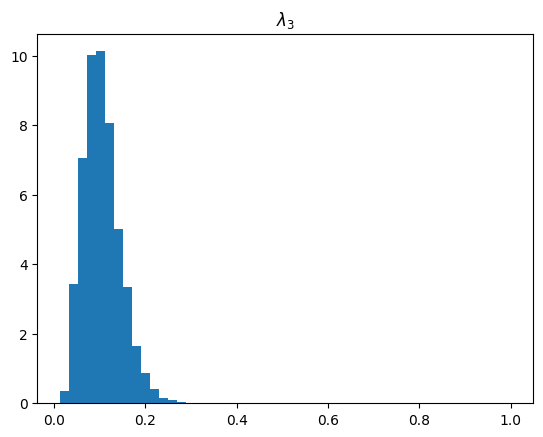
\includegraphics[width = 10 cm]{Figures/histograma3_3.png} 
  \caption{Histograma de la marginal de la posterior de $\lambda_3$.}
  \label{Fig. 3.04}
\end{figure} 
\begin{figure}[H] 
  \centering 
  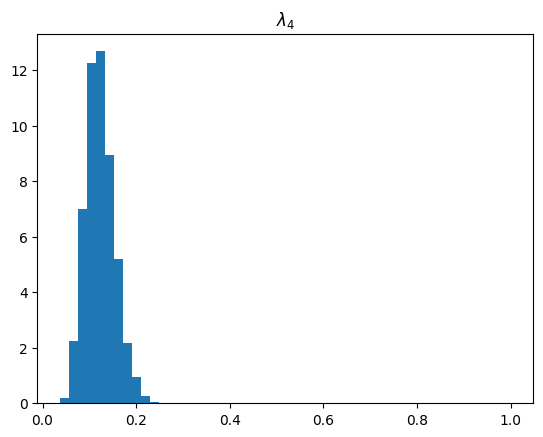
\includegraphics[width = 10 cm]{Figures/histograma3_4.png} 
  \caption{Histograma de la marginal de la posterior de $\lambda_4$.}
  \label{Fig. 3.05}
\end{figure} 
\begin{figure}[H] 
  \centering 
  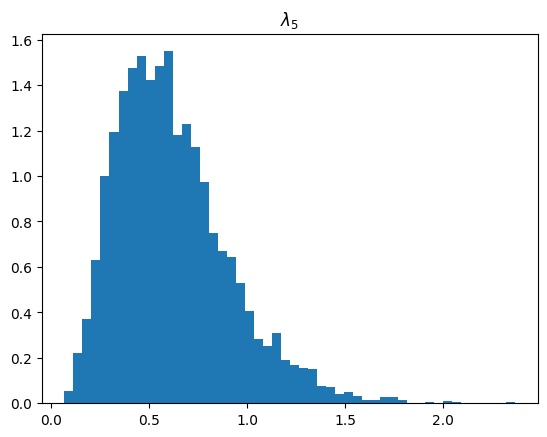
\includegraphics[width = 10 cm]{Figures/histograma3_5.png} 
  \caption{Histograma de la marginal de la posterior de $\lambda_5$.}
  \label{Fig. 3.06}
\end{figure} 
\begin{figure}[H] 
  \centering 
  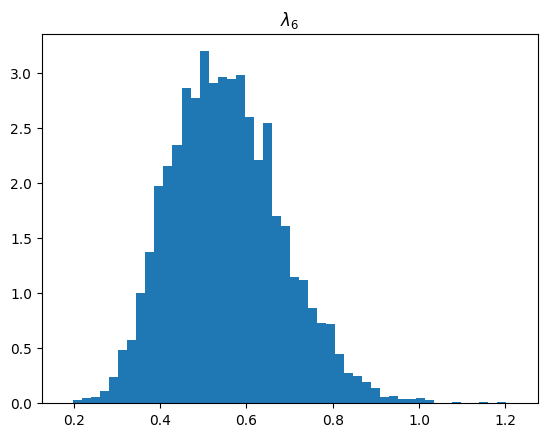
\includegraphics[width = 10 cm]{Figures/histograma3_6.png} 
  \caption{Histograma de la marginal de la posterior de $\lambda_6$.}
  \label{Fig. 3.07}
\end{figure} 
\begin{figure}[H] 
  \centering 
  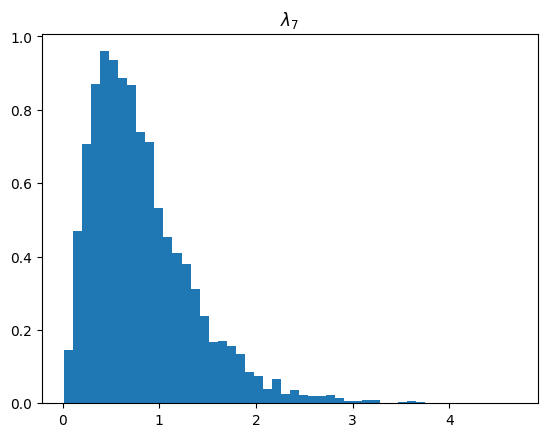
\includegraphics[width = 10 cm]{Figures/histograma3_7.png} 
  \caption{Histograma de la marginal de la posterior de $\lambda_7$.}
  \label{Fig. 3.08}
\end{figure} 
\begin{figure}[H] 
  \centering 
  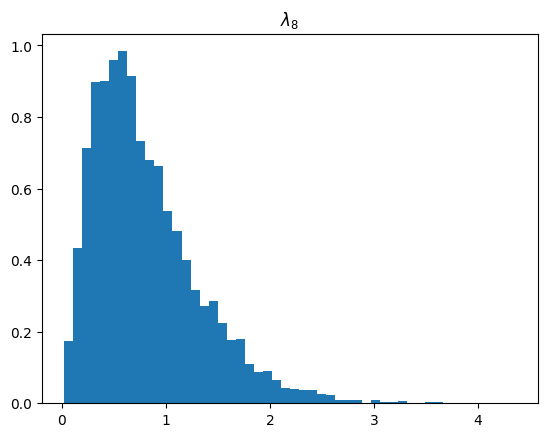
\includegraphics[width = 10 cm]{Figures/histograma3_8.png} 
  \caption{Histograma de la marginal de la posterior de $\lambda_8$.}
  \label{Fig. 3.09}
\end{figure} 
\begin{figure}[H] 
  \centering 
  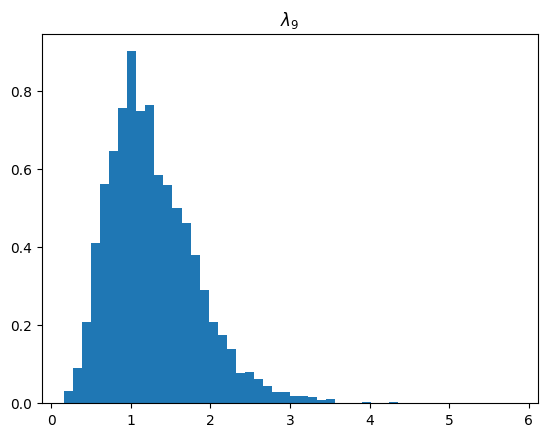
\includegraphics[width = 10 cm]{Figures/histograma3_9.png} 
  \caption{Histograma de la marginal de la posterior de $\lambda_9$.}
  \label{Fig. 3.10}
\end{figure} 
\begin{figure}[H] 
  \centering 
  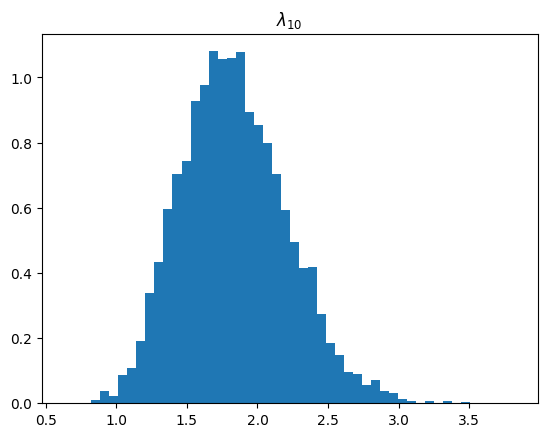
\includegraphics[width = 10 cm]{Figures/histograma3_10.png} 
  \caption{Histograma de la marginal de la posterior de $\lambda_10$.}
  \label{Fig. 3.11}
\end{figure} 

\end{solution}

\begin{thebibliography}{9}

    \bibitem{Casella}
    Robert, C. P., Casella, G., and Casella, G. (1999). Monte Carlo statistical methods (Vol. 2). New York: Springer.

    % \bibitem{Wasserman}
    % Wasserman, L. (2004). All of statistics: a concise course in statistical inference (p. 413). New York: Springer.
    
\end{thebibliography}
      




    \end{document}